\documentclass[oneside, class=book, 12pt, crop=false]{standalone}

\usepackage{../dissertationstyle}

\bibliography{../personal}

\begin{document}

\ifstandalone
  \setcounter{chapter}{3}
  \chapter{Evaluation}
\fi
\resetfigpath{evaluation}
% write about:
% individual metric capabilities, check in implementation for combos
% peak metric success
% how each metric and peak metric success were affected by variations
% plot graph of noise vs time

In this chapter, we evaluate the success of the project, with reference to the requirements given in Table \ref{table:requirements}. We also explore the absolute performance of the system, as well as comparative success. 

\section{Requirements Analysis Revisited}

All of the non-extension requirements were successfully completed:

\begin{itemize}
  \item
    \textbf{Calculators for each of the 5 proposed metrics}

    As explained in Chapter \ref{chapter:implementation}, each of the metrics were implemented in such a way that they successfully capture information outlined in Chapter \ref{chapter:introduction}. We will see evidence of this success later in the chapter.

  \item
    \textbf{Similarity scorers for each of the 5 proposed metrics}

    Again, we have seen that we were able to implement similarity scorers for each of the metrics, and the evidence we see later in this chapter tells us that these capture sensible notions of similarity.

  \item
    \textbf{Additional of optional variation to input data}

    As seen in Section \ref{sec:transformations}, we are able to add variation to input data such that we are able to somewhat realistically mimic sonic effects that could be perceived in other recordings.

  \item
    \textbf{Code to automatically perform evaluation based on a plan}

    As we will see in the next section (TODO: add reference), we were was able to implement a framework for evaluating the system given a number of parameters, allowing for easy gathering of data.

  \item
    \textbf{Data synthesis engine to generate test piano data}

    As seen in Section \ref{sec:datasynthesis}, we implemented an engine that was able to parse scores and synthesise audio with added variation that aided in development of the core system.

  \item
    \textbf{Data synthesis engine to generate test data from other instruments}

    This was an extension requirement, and was unable to be completed. Generating good test data from other instruments would require more than a surface level understanding of the instrument, and I did not have enough time to both do this research and implement a data synthesis engine based on my findings.

  \item
    \textbf{Gathering of real-world piano performances}

    As outlined in Section \ref{sec:datacollection}, we successfully gathered a total of 32 (TODO: change if got more) real-world piano performances, using a range of piano pieces that cover different techniques (and thus sound different).
\end{itemize}

\section{Evaluation of Metrics}

In this section, we discuss how each metric and metric combination were evaluated, as well as the framework developed to aid implementation.

To evaluate our system, we only really care about one statistic: does the system guess the correct performer given one distinguished performance, and a set of performances where one is by the same performer as the distinguished performance. Furthermore, since our dataset is relatively small, it was important to try and use this dataset in many ways to gather enough evaluation information. For these reasons, in order to evaluate the system for a set of performances $P$ containing two performances of the same piece for each pianist, we do the following:

\begin{itemize}
  \item
    Initialise a counter $c$ to 0

  \item
    Choose each performance from $P$ as the `distinguished' performance $p$ in turn

    \begin{itemize}
        

      \item
        Calculate metrics for all of the performances in $P$

      \item
        Calculate the mean similarity over each of the metrics between the distinguished performance $p$ and  $P \setminus \{p\}$

      \item
        Take the system's guess $p'$ as the performance with the highest mean similarity
      \item
        If $p$ has the same performer as $p'$, increment $c$
    \end{itemize}

  \item
    The success for $P$ is then the $c$ divided by the total number of guesses our system made, which is $|P|$.
\end{itemize}

We can then extend this if we have multiple collections $P$ by simply taking the mean success, weighted by the size of each collection.

It should be noted here that it may seem like we are inflating our results, since if we have two performances $p_1$ and $p_2$ by the same performer, we have one instance where we choose $p_1$ to be our distinguished performance, and another where we choose $p_2$, and by symmetry of our similarity scorers it may seem like this is a bad idea. However, there could be a third performance $p_3$ that $p_2$ has the highest aggregate similarity with, but does not have the highest aggregate similarity with $p_1$, so we are not inflating our results.

This method allows us to get a lot of evaluation data from just a few performances, for a set of performances $P$ we get a granularity of $\frac{1}{|P|}$. In our case, each of our sets of performances have 8 performances each, and we have 4 different pieces, which gives us a granularity of $\frac{1}{32}$.

We can go even further, and find what success we need for a result to be statistically significant. For a set of performances $P$, if our system guessed at random, we would have a $\frac{1}{|P|}$ probability of guessing correctly. Now, suppose we have $n$ sets of performances $P_1, \ldots, P_n$. To match our dataset, we will assume that the $P_i$ all have the same size. This means that we can model the number of successful guesses of our system as a random variable modelled by a binomial distribution $X \sim B(n|P_i|, \frac{1}{|P_i|})$. At a significant level of $p$, we then just need to find the least $m$ such that $P(X \geq m) \leq p$.

For our dataset, we have $n=4$, $|P_i| = 8$, and we set $p$ at 0.05. We then find that $P(X \geq 6) = 0.096$ (2 s.f.) and $P(X \geq 7) = 0.040$ (2 s.f.), so our critical value is 7. This means we only need to get 7 successful trials, or a success of 0.22 (2 s.f.) for our system to be statistically significantly better than random.

\subsection{Evaluation Framework}

To speed up evaluation, it was important to easily be able to evaluate the entire dataset (as described earlier) on any combination of metrics, and with any number of transformations. Furthermore, the evaluation should be reasonably fast since we need to evaluate the dataset over a very large parameter space.

For this reason, we implemented an \texttt{evaluate\_metrics} function in \texttt{src/classifier/evaluation.py} that, given a list of metric calculators and a list of transformations, evaluated the entire dataset and returned its success. Furthermore, a number of caching mechanisms were implemented that were vital to the success of evaluation: the time it would have taken to evaluate the system would have been nearly infeasible without them. Calculating the metrics and similarities involves rather expensive operations, so metrics were cached and onset functions were cached, since onset functions are quite expensive to compute and underpin a lot of the metric calculators and similarity scorers.

\section{Metric Performance}

In this section we look at the performance of each metric and particular metric combinations, as well as the effects of transformations on the results.

\subsection{Individual Metrics}

A table of the success' for each metric is given in Table \ref{table:metric results}. 

\begin{table}[h]
    \centering
    \begin{tabular}{cc}
        \textbf{Metric}&\textbf{Success} (2 s.f.) \\
        \midrule[0.15em]
        Tempo variation over time&0.31 \\
        Dynamics over time&0.56 \\
         Chroma vector extraction&0.50 \\
         Note offsets&0.66 \\
         Timbre extraction&0.25\\
    \end{tabular}
    \caption{Individual metric results}
    \label{table:metric results}
\end{table}

Whilst the results for individual metrics are not stellar, they are all statistically significant (at $p=0.05$), which shows that, to some extent, each of the metrics was devised and implemented sensibly. TODO: show tempo graphs. Three metrics, however, performed significantly better than the other two: dynamics over time, chroma vector extraction, and note offsets. The metric that performed the worst was the timbre extraction metric, which was theorised at the start to not have the most potential. It is possible that the timbre extraction might not even be significantly better than random on its own merit: as explained in Section \ref{sec:timbre metric}, our estimation of normalising the MFCCs on pitch is only crude, and so the performance of this metric might instead be proxying the performance of the chroma metric.

%TODO: remember that poor performance of the tempo metric might be bad scaling

\subsection{Metric Combinations}

Whilst individual metrics were not able to perform extremely well, much better performance could be attained by combining multiple metrics together. For example, as theorised in Section \ref{sec:chroma similarity}, the combination of both the chroma and dynamics metrics were able to achieve a success of 0.59 (2 s.f.), due to there being some pieces/performers that the chroma metric was good at differentiating, and some distinct pieces/performers that the dynamics metric was good at differentiating.

By just combining two metrics, the best success attained was the combination of the dynamics and offsets metrics (the two highest performing individual metrics), achieving a success of 0.75 (2 s.f.).

Even better results could be attained by combining 3 or 4 metrics. The two best metric combinations were found by combining the chroma, dynamics, and offsets metrics, and by combining the chroma, dynamics, offsets, and timbre metrics, both achieving a success of 0.78 (2 s.f.). Since the only difference between these two sets of metrics is the addition of the timbre metric, this provides even more evidence that the timbre metric is not that useful. In fact, combining any other metric $M$ with the timbre metric did not result in a different success to having just $M$ by itself.

Interestingly, combining all 5 metrics only resulted in a success of 0.69 (2 s.f.), which implies that the tempo metric is somehow antagonistic with some other metrics in our system.

By investigating further, we find that only the chroma metric received an increase in success when combined with the tempo metric (increasing from 0.50 to 0.59 (2 s.f.)), whereas all other metrics (ignoring timbre) took a decrease in success of 28\% and 10\% for dynamics and note offsets respectively. So, even though there is some affinity between the chroma and tempo metrics, this is not enough to outweigh the antagonism between the tempo metric and the dynamics and note offsets metrics, resulting in a decrease in performance when we use all 5 metrics.

\subsection{Performance under Transformations}

The performance of the metrics under noise and reverb transformations is somewhat interesting. In Table \ref{table:transformation results}, we give the success for each individual metric under each combination of transformations, including no transformations (for completeness, this is just the same data we store in Table \ref{table:metric results}).

\begin{table}[h]
    \centering
    \begin{tabular}{c|cc}
        \textbf{Transformation}&\textbf{Metric}&\textbf{Success} (2 s.f.) \\
        \midrule[0.15em]
        \multirow{5}{*}{None} &Tempo variation over time&0.31 \\ \cline{2-3}
                              &Dynamics over time&0.56 \\ \cline{2-3}
                              &Chroma vector extraction&0.50 \\ \cline{2-3}
                              &Note offsets&0.66 \\ \cline{2-3}
                              &Timbre extraction&0.25\\ \midrule[0.1em]
        \multirow{5}{*}{Noise} & Tempo variation over time & 0.31 \\ \cline{2-3}
                               &Dynamics over time & 0.47 \\ \cline{2-3}
                               &Chroma vector extraction & 0.53 \\ \cline{2-3}
                               &Note offsets & 0.63 \\ \cline{2-3}
                               &Timbre extraction & 0.25 \\ \midrule[0.1em]
        \multirow{5}{*}{Reverb} & Tempo variation over time & 0.38 \\ \cline{2-3}
                                &Dynamics over time & 0.53 \\ \cline{2-3}
                                &Chroma vector extraction & 0.38 \\ \cline{2-3}
                                &Note offsets & 0.69 \\ \cline{2-3}
                                &Timbre extraction & 0.25 \\ \midrule[0.1em]

        \multirow{5}{*}{Noise + Reverb} & Tempo variation over time & 0.41 \\ \cline{2-3}
                                &Dynamics over time & 0.50 \\ \cline{2-3}
                                &Chroma vector extraction & 0.41 \\ \cline{2-3}
                                &Note offsets &  0.63\\ \cline{2-3}
                                &Timbre extraction & 0.25 \\ 
        
    \end{tabular}
    \caption{Individual metric results under various transformations}
    \label{table:transformation results}
\end{table}

%TODO: hypothesis tests

As we can see, introduction of transformations causes some performances to have a reduction in performance, but bolsters others. The timbre metric remains completely unaffected by any transformation, which again implies that it is not much better than random.

When looking into the performance of metric combinations, we see that the noise transformation actually results in a better peak success: 0.81 (2 s.f.) with the same best metric combinations for no transformations. When adding the reverb transformation, our peak success decreases, only being able to attain a peak success of 0.69 (2 s.f.), which is no better than the success obtained by the note offsets metrics on its own. Interestingly, we can see that the chroma metric took a large performance hit, and none of the best metric combinations include the chroma metric. Finally, applying noise and then reverb allows us to attain a peak success of 0.75 (2 s.f.) with numerous metric combinations, but none including the chroma metric.

These results seem counter-intuitive, since we seem to be gaining performance by adding noise into our system. The graph in Figure \ref{fig:noiseplot} shows how the best and worst metric performance changes as we increase the amplitude of the noise that we add.

% TODO: change this plot to its actual one
\begin{figure}[h]
    \centering
    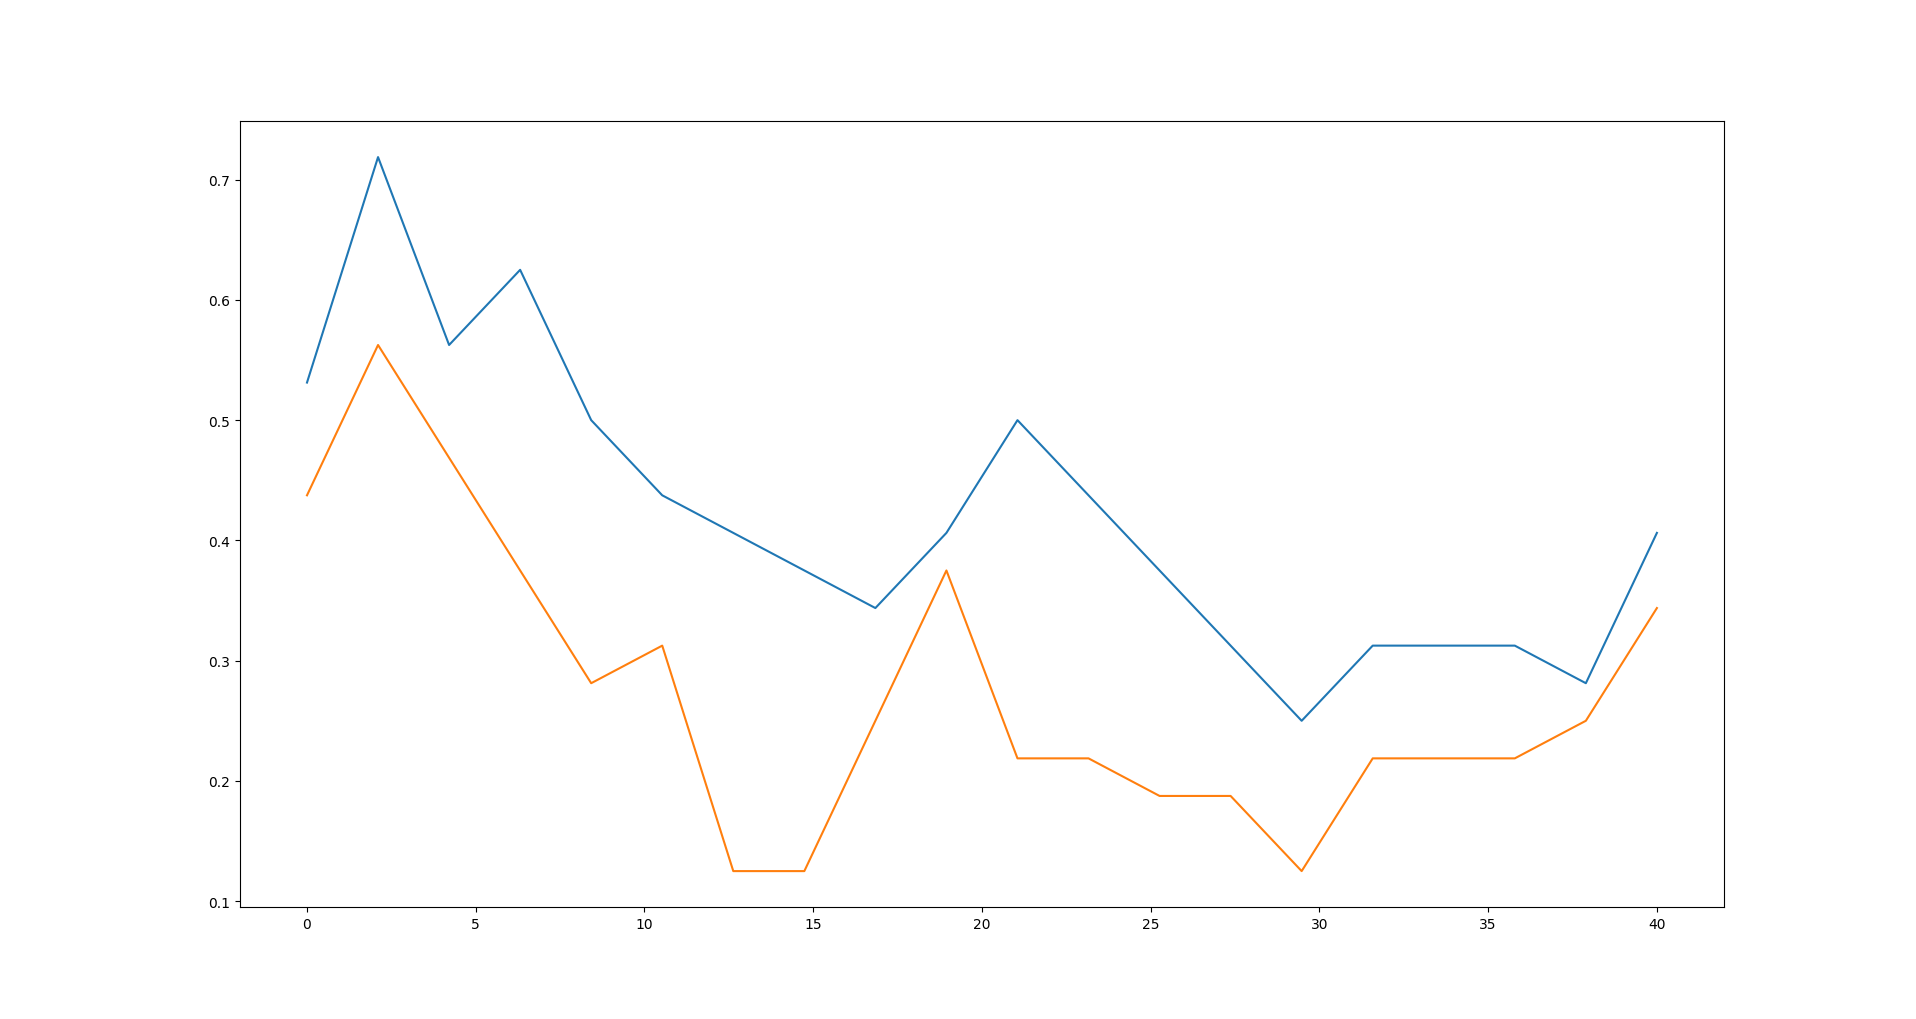
\includegraphics[scale=0.3]{noiseplot}
    \caption{Best and worst metric performance against noise amplitude}
    \label{fig:noiseplot2}
\end{figure}

Although the peak performance varies (and sometimes increases), there is a general trend of it decreasing, although it is impressive that the system is still able to perform reasonably well under very amplified noise. The worst performance, however, suffers tremendously, such that the system is sometimes worse than random (which occurs at a success of 0.125), and is even capable of being unable to correctly identify a single performer at certain points. This indicates that the noise is somehow acting adversarially to our system, since otherwise we would not expect the system to become worse than random.









\ifstandalone
  \printbibliography
\fi
    
\end{document}
